

\boxx{
	\paragraph{Learning objectives}
	\itex{
		\item Distinguish between quantity demanded and demand, 	and explain what determines demand.
		\item  Distinguish between quantity supplied and supply, and 	explain what determines supply.
		\item  Explain how demand and supply determine price and 	quantity in a market, and explain the effects of changes 	in demand and supply.
	}
	%Please read the corresponding chapter of \cite{Parkin2012Economics} --- Either the \textit{Economics }version or the \textit{Microeconomics} version.
}


\boxx{
	Recommended readings:
	\itex{
		\item \citet[ch. 3]{Shapiro2022Principles}
%		\item \citet[pt. II, ch. 7, 8, 34]{Mankiw2020Principles} 
	}	
}

\pbn
\section{Introduction: What is a market?}

\subsection{The problem of value: The Water-Diamond Paradox}

\zitat{``Water is clearly important. We literally can't live without it. Yet you can get water in your apartment in New York without paying for it. On modern Roman streets you can wash your hands or bathe your dog at any old fire hydrant. In the office and in the dorm you can drink water from the fountain down the hall.
	
	Diamonds are different. You can live without diamonds. Yet they are very expensive, valued extremely highly per ounce in the marketplace.
	
	Notice how strange this is - how a good such as a diamond, which is beautiful but inessential, could be so much more expensive per ounce than an essential and not necessarily beautiful good, such as water. The case is called `the water/diamond paradox.' It is the first and the deepest question of value. What, after all, determines the value of things?'' --- \href{http://www.theeconomicconversation.com/book/ch5.1.php}{http://www.theeconomicconversation.com}}



\exex{From moral to amoral theories of value}{
	Discuss the water-diamond paradox. Can you think of similar examples of goods that have a high price but no \textit{real value}. Also discuss, what is the \textit{value of a good} when its not the price?
	%	
	%	Feel free to read this section \webbig\url{http://www.theeconomicconversation.com/book/ch5.2.php} wherein we get the lesson that demand and 
}

\pbn
\subsection{Elements of a market}
\itex{
	\item A market is any arrangement that brings buyers and sellers together.
	\item A \textbf{market} might be a physical place or a group of buyers and sellers spread around the world who never meet.
	\item In this chapter, we study a \textbf{competitive market} that has so many buyers and so many sellers that no individual buyer or seller can influence the price.
	\item \textbf{Quantity demanded} is the amount of a good, service, or resource that people are willing and able to buy during a specified period at a specified price.
	The quantity demanded is an amount per unit of time. For example, the amount per day or per month.
	\item \textbf{Supply and demand} are the forces that make market economies work because they determine prices in a market economy. 
	\item \textbf{Prices}, in turn, allocate the economy’s scarce resources. 
	\item The model of the market based on supply and demand, like any other model, is based on a series of assumptions.}

\pbn
\boxx{
	\subsubsection*{Assumptions of the classical model}
	The classical model of supply and demand in free markets is basically based on the following assumptions (also see: exercise \ref{sol:Magic of the price system}):
	
	\itex{
		\item  Many buyers and sellers
		\item  Homogeneous products
		\item  Perfect information
		\item  Free entry and exit
		\item  Perfect mobility of factors of production 
		\item  Profit maximization
		\item  No externalities
}}

\pbn
\section{Demand}

\subsection{The law of demand}
Other things remaining the same,
\itex{\item 	If the price of the good rises, the quantity demanded of that good decreases.
	\item	If the price of the good falls, the quantity demanded of that good increases.
}

\pbn
\exex{Greed}{
	Watch Gordon Gekko's ``Greed is good'' speech taken from the movie
	\textit{Wall Street} (1987):
	\begin{center}
		\includegraphics[width=.4\linewidth]{$HOME/Dropbox/hsf/pic/micro/wallstreet}
	\end{center}
	\tvbig \url{https://youtu.be/VVxYOQS6ggk}
	and discuss the relationship of \textit{greed} and the \textit{law of demand}.
}

\pbn
\subsection{Demand schedule and demand curve}
Demand is the relationship between the quantity demanded and the price of a good when all other influences on buying plans remain the same. 
Demand is illustrated by a demand schedule and a demand curve.
The demand curve shows the relationship between price and quantity demanded

\textbf{Rachel's demand schedule}

	\begin{center}
		\begin{tabularx}{.5\textwidth}{CC}
			\toprule
			Price of milk per litre (\euro) & Quantity of mild demanded (litres per month) \\\midrule 
			.00&  20\\ 
			.1&18  \\  
			.2&16  \\  
			.3&  14\\  
			.4&  12\\  
			.5&  10\\  
			.6&  8\\  
			.7&  6\\  
			.8&  4\\
			.9& 2\\\bottomrule 
		\end{tabularx} 	
	\end{center}



\begin{center}
	\includegraphics[width=0.7\linewidth]{../../../pic/micro/rachel}
\end{center}


\pbn
\subsection{Market demand versus individual demand}
\itex{\item Market demand refers to the sum of all individual demands for a particular good or service.
	\item		Graphically, individual demand curves are summed horizontally to obtain the market demand curve. }

\begin{minipage}[t]{0.4\textwidth}
	\includegraphics[width=\textwidth]{../../../pic/micro/rachel2}
\end{minipage}
\begin{minipage}[t]{0.4\textwidth}
	\includegraphics[width=\textwidth]{../../../pic/micro/lars}
\end{minipage}

\exex{Aggregate individual demand}{
	Sketch the market demand for milk, i.e., the sum of the demands of all the buyers in a market.
}
\solx{Aggregate individual demand}{
	\begin{center}
		\includegraphics[width=.6\textwidth]{../../../pic/micro/rachel_lars}
	\end{center}\label{fig:demand_milk}
}

\pbn
\subsubsection{Movements along the curve versus shifts}
\itex{\item Movements along the demand curve are caused by a change in the price of the product.
	\item Ceteris paribus condition -- other factors affecting demand are held constant so that we can analyze the effect of a change in price on demand.
	\item  		A shift in the demand curve is caused by a factor affecting demand other than a change in price. }

\pbn
\exex{Sources of demand}{
	\itex{\item Can you think of factors that change demand for a given price? Do the prices of other goods play a role?
		\item A \textbf{substitute} is a good that can be consumed in place of another good.
		For example, apples and oranges are substitutes.
		\item A \textbf{complement} is a good that goes well with another good. For example, sausages and mustard or fish and chips.
		\item Fill in the blanks:\\
		The demand for a good \rule{4em}{0.15mm} (increases/decreases) if the price of one of its substitutes rises.\\
		The demand for a good \rule{4em}{0.15mm} (increases/decreases)  if the price of one of its substitutes falls.\\
		The demand for a good \rule{4em}{0.15mm} (increases/decreases)  if the price of one of its complement rises.\\
		The demand for a good \rule{4em}{0.15mm} (increases/decreases)  if the price of one of its complement falls.\\
		A rise in the expected future price of a good  \rule{4em}{0.15mm} (increases/decreases) the current demand for that good.\\
		A fall in the expected future price of a good  \rule{4em}{0.15mm} (increases/decreases) current demand for that good.\\
		\item A \textbf{normal good} is a good for which the demand increases if income increases and demand decreases if income decreases.
		\item An \textbf{inferior good} is a good for which the demand decreases if income increases and demand increases if income decreases.
		\item Can you give examples for normal and inferior goods.
		\item Fill in the blanks:\\
		When income is expected to increase in the future, or when credit is easy to get and the cost of borrowing is low, the demand for some goods  \rule{4em}{0.15mm} (increases/decreases).\\
		When income is expected to decrease in the future, or when credit is hard to get and the cost of borrowing is high, the demand for some goods  \rule{5em}{0.15mm} (increases/decreases).\\
		\item Is the following statement true or false:\\
		Changes in expected future income and the availability and cost of credit has the greatest effect on the demand for big ticket items such as homes and cars.
}}


\pbn
\subsubsection{Movements along the demand curve}
Suppose the price of milk falls.
\itex{\item More milk will be demanded because of income and substitution effects.
	\item	\textbf{The income effect.} Assume that incomes remain constant. Then a fall in the price of milk means that consumers can now afford to buy more with their income. 
	\item \textbf{The substitution effect.} Milk is lower in price compared to other similar products so some consumers will choose to substitute the more expensive drinks with the now cheaper milk.
}

\pbn
\subsubsection{Shifts in the demand curve}
A shift in the demand curve---to the left or right---is caused by any change that alters the quantity demanded at every given price.

\paragraph{Shifting factors:}
\itex{\item Price of related goods: substitutes and complements
	\item Income: A lower income means consumer can spend less in total, so they spend less on some --and probably most-- normal goods but more on inferior goods.
	\item preferences
	\item number of buyers (population)
	\item advertising
	\item expectation of consumers if demand is influenced by expectations of future income and future prices
	\item ... 
}

%\begin{center}
%	\includegraphics[width=1.0\textwidth]{../../../pic/micro/sdshift}
%\end{center}\label{fig:sdshift}


\pbn
\exex{Three demand curves}{
	Draw a plot with three demand curves. One curve should represent an economy in an economic booming phase, one in en economic downturn and one in between.\medskip
	
	\begin{center}
		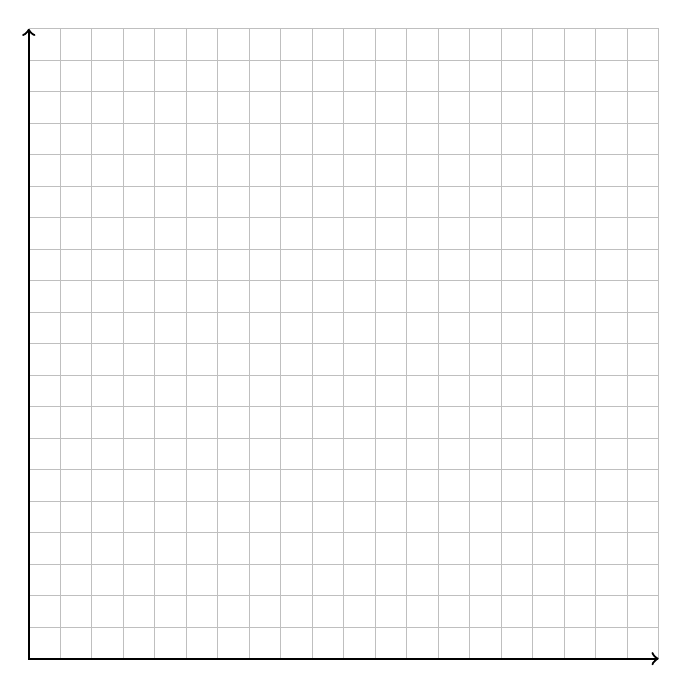
\begin{tikzpicture}[scale=.4]
			%			[yscale=.5,xscale=1.9]
			\draw [color=gray!50]  [step=10mm] (0,0) grid (20,20);
			\draw[thick,<->] (0,20)--(0,0)--(20,0);
			%	\draw[blue, thick,-] (0,10) --(30,0); 
			%%	\node [above right] at (30,10) {$Q^S$};
			%	\draw[red, thick,-] (0,1) --(30,11); 
			%	\node [above right] at (30,0) {$Q^D$};
			%	\draw[blue, thick,->] (1,5) --(4/3,4); 
			%	\node [below left] at (0,0) {$ $};%Origin
			%	\draw[red, dashed]  (0,4)   -- (4/3,0)  ;
			%	\draw[red, dashed]  (0,8)   -- (8/3,0)   ;
			%	\tkzDefPoint(1,1){A}
			%	\tkzLabelPoint[right,font=\tiny](A){(100,100)}
			%	\tkzDefPoint(1,5){B}
			%	\tkzLabelPoint[right,font=\tiny](B){(500,100)}
			%	\tkzDefPoint(2/3,2){C}
			%	\tkzLabelPoint[right,font=\tiny](C){(200,$\frac{200}{3}$)}
			%	\tkzDefPoint(4/3,4){D}
			%	\tkzLabelPoint[right,font=\tiny](D){(400,$\frac{400}{3}$)}
			%	\foreach \n in {B,A,C,D}
			%			\node at (\n)[circle,fill,inner sep=1.5pt]{};
			%			\draw[dotted] (0,0)--(4,4) node[left]{$x=y$};
		\end{tikzpicture}
		%	\captionof{figure}{Changes in consumption}\label{fig:cic}
	\end{center}	
}






	


\section{Supply}

\subsection{The law of supply} 
Other things remaining the same, it holds that:
\itex{\item 	If the price of a good rises, the quantity supplied of that good increases.
	\item If the price of a good falls, the quantity supplied of that good decreases.}

\paragraph{Supply: Definitions}
\itex{\item \textbf{Quantity supplied} is the amount of a good that sellers are willing and able to sell. 
	\item The \textbf{supply schedule} is a table that shows the relationship between the price of the good and the quantity supplied.
	\item The \textbf{supply curve }is the graph of the relationship between the price of a good and the quantity supplied }


\pbn
\subsection{Supply schedule and supply curve}
The following supply curve shows the relationship between price and quantity supplied of Richard who is a farmer.

\begin{minipage}{0.5\textwidth}
	\scriptsize
	\begin{center}
		\begin{tabularx}{.9\textwidth}{ CC}
			\toprule
			Price of milk per litre (\euro) & Quantity of mild supplied (litres per month) \\\midrule 
			.00&  0\\ 
			.1&0 \\  
			.2&2  \\  
			.3&  4\\  
			.4&  6\\  
			.5&  8\\  
			.6&  10\\  
			.7&  12\\  
			.8&  14\\
			.9& 16\\
			1&18\\\bottomrule 
		\end{tabularx} 	
	\end{center}
\end{minipage}
\begin{minipage}{0.5\textwidth}
	\begin{center}
		\includegraphics[width=.9\textwidth]{../../../pic/micro/farmer}
	\end{center}
\end{minipage}

\pbn
\subsection{Market supply versus individual supply}
Market supply refers to the sum of all individual supplies for all sellers of a particular good or service.
\begin{center}
	\begin{tabular}{cccc}\toprule
		Price of milk per litre (\euro) & Richard + & Megan= & Market \\ \midrule
		0 & 0 & 0 & 0 \\ 
		.1 & 0 & 1 & 1 \\ 
		.2 & 2 & 2 & 4 \\ 
		.3 & 4 & 3 & 7 \\ 
		.4 & 6 & 4 & 10 \\ 
		.5 & 8 & 5 & 13 \\ 
		.6 & 10 & 6 & 16 \\ 
		.7 & 12 & 7 & 19 \\\bottomrule	\end{tabular} 
\end{center}\label{tab:supply_milk}


\pbn
\begin{center}
	\includegraphics[width=.6\textwidth]{../../../pic/micro/aggsupply}
\end{center}


\subsubsection{Movements along the curve versus shifts}
\itex{\item The supply curve shows how much producers offer for sale at any given price, holding constant all other factors that may influence producers’ decisions about how much to sell.
	
	\item	A change in any of these other factors (other than a change in prices) shifts the supply curve to the left or to the right.}

\pbn
\subsubsection{Shifts in the supply curve }
\itex{\item Profitability of other goods in production and prices of goods in joint supply.
	\item 	Technology.
	\item Number of Sellers
	\item 	Natural/Social Factors such as the weather and changing attitudes.
	\item Input prices – the prices of the factors of production.
	\item 		Expectations of producers about the future state of the market.
	\item 	A change in the number of sellers in the market.
	\item Prices of Resources and Other Inputs: Resource and input prices influence the cost of production. And the more it costs to produce a good, the smaller is the quantity supplied of that good.
	\item \textbf{Expected Future Prices:}
	Expectations about future prices influence supply.
	Expectations of future prices of resources also influence supply.
	\item Productivity which is output per unit of input. An increase in productivity lowers costs and increases supply. 
	\item \dots}

\pbn
\exex{Prices of Related Goods in Production}{
	\itex{\item A change in the price of one good can bring a change in the supply of another good.
		\item A \textbf{substitute in production} is a good that can be produced in place of another good.\\
		\item Give examples for goods that are substitutes in production.
		\item 
		Fill in the blanks:\\
		The quantity supplied of a good 
		\xblackout{increases}(increases/decreases) if the price of one of its substitutes in production falls.\\
		The quantity supplied of a good 
		\xblackout{decreases}(increases/decreases) if the price of one of its substitutes in production rises.\\
		The quantity supplied of a good \xblackout{increases}(increases/decreases)  if the price of one of its complements in production rises.\\
		The quantity supplied of a good \xblackout{decreases}(increases/decreases)  if the price of one of its complements in production falls.
		
	}
}

\solx{Prices of Related Goods in Production}{
	decreases, increases, decreases, increases
}
%
%\begin{center}
%	\includegraphics[width=1.0\textwidth]{../../../pic/micro/supplyshift.png}
%\end{center}

\pbn
\section{Market equilibrium}


\boxx{\textbf{Equilibrium Price}
	\itex{\item	The price that balances quantity supplied and quantity demanded. 
		\item Graphically, this is the price at which the supply and demand curves intersect.}}
\boxx{\textbf{Equilibrium Quantity}
	\itex{\item	The quantity supplied and the quantity demanded at the equilibrium price. 
		\item	Graphically, this is the quantity at which the supply and demand curves intersect.  	}}

\paragraph{What is an equilibrium}
In economics, economic equilibrium is a situation in which economic forces such as supply and demand are balanced and in the absence of external influences the (equilibrium) values of economic variables will not change.

\textbf{When we look on supply and demand:} Price adjustments lead to an alignment of the
quantities of goods supplied and demanded.

\pbn

\begin{figure}\centering
	\includegraphics[width=.6\textwidth]{../../../pic/micro/equilibrium}
	\caption{Market equilibrium of supply and demand}
\end{figure}

\pbn
\exex{Demand and Supply}{
	Given the demand function
	$$x(p) = -\frac{3}{4}p + 300$$
	and the supply function
	$$x_S(p) = \frac{5}{4}p -100$$
	Determine the equilibrium market price and quantity both graphically and algebraically.
}
\pbn


\solx{Demand and Supply}{
	To find the equilibrium, a.k.a. the intersection of the two functions, you need to solve the system of equations by solving both both equations fo either $x$ or $p$ and set both equal. To substitute for $x$ you should calculate
	\begin{align*}
		-\frac{3}{4}p + 300&=\frac{5}{4}p -100\\
		p^*&=200\\
		\textnormal{and } x^*&=150
	\end{align*}
	To substitute for $p$ you need to solve both equations for $p$:
	$$x = x(p) = -\frac{3}{4}  + 300 \Leftrightarrow p(x) = -\frac{4}{3}x +400$$
	$$x_S(p) = \frac{5}{4}p -100 \Leftrightarrow p_S(x) = \frac{4}{5} x +80$$
	and calculate
	\begin{align*}
		-\frac{4}{3}x +400&=\frac{4}{5} x +80\\
		x^*&=150\\
		\textnormal{and } p^*&=200
	\end{align*}
	The equilibrium market price and quantity is in $x=150$ and $p=200$.
	\begin{center}
		\includegraphics[width=.45\linewidth]{$HOME/Dropbox/hsf/pic/mas/exe22}
	\end{center}
}


\pbn
\begin{figure}\centering
	\includegraphics[width=.7\textwidth]{../../../pic/micro/exsupply}
	 \caption{Markets not in equilibrium}
\end{figure}

\pbn
\subsubsection{Supply > Demand (Surplus / Excess)}
\itex{\item If price > equilibrium price, 
	\item then quantity supplied > quantity demanded.  
	\item There is excess supply or a surplus.  
	\item Suppliers will lower the price to increase sales, thereby moving towards equilibrium.
}

\subsubsection{Supply < Demand (Shortage)}
\itex{\item	If price < equilibrium price, the quantity demanded > the quantity supplied.  
	\item There is excess demand or a shortage. 
	\item Suppliers will raise the price due to too many buyers chasing too few goods, thereby moving toward equilibrium.	
}

\pbn
\paragraph{Prices as signals}
\textbf{Law of supply and demand}
\itex{\item The price of any good adjusts in order to bring the quantity supplied and the quantity demanded for that good into balance.
	\item The main function of a price in a free market is to act as a signal to both buyers and sellers. 
	\item Buyers check whether they are willing to pay the price of an item, i.e., if the benefits (\textit{utility}) exceeds the costs. 
	\item Sellers examine whether the price of a good exceeds the costs of production.
}

\paragraph{Three steps to analyzing changes in equilibrium}
\enux{\item Decide whether the event shifts the supply or demand curve (or both).
	\item Decide whether the curve(s) shift(s) to the left or to the right.
	\item Use the supply and demand diagram to see how the shift affects equilibrium price and quantity.}	


\pbn
\paragraph{How an increase in demand affects the equilibrium}
\begin{center}
	\includegraphics[width=.8\textwidth]{../../../pic/micro/indemand}
\end{center}


\paragraph{How a decrease in supply affects the equilibrium}
\begin{center}
	\includegraphics[width=.8\textwidth]{../../../pic/micro/desupply}
\end{center}	



\pbn
\exex{Effects of a new fertilizer}{
	Assume that a new fertilizer dramatically increases the number of potatoes that can be harvested with no additional labor or machinery. Also assume that this fertilizer does not affect wheat farming and that people are satisfied to eat either potatoes or bread made from wheat flour.
	
	Illustrate for both markets, potato and bread, how demand, supply, the equilibrium prices, and quantities change due to the new fertilizer.
}

\pbn

\solx{Effects of a new fertilizer}{
	\begin{center}
		\includegraphics[width=.8\textwidth]{../../../pic/micro/fertilizer}
	\end{center}	\tiny Source: Advanced Placement Economics Microeconomics: Teacher Resource Manual Council for Economic Education, New York, N.Y.
}

\pbn
\exex{Effects of a study on coffee}{
	Assume new studies show that coffee is worse for people’s health than tea and that more people use cream in coffee than in tea. 
	
	Illustrate the changes in the markets of coffee, tea, and cream.
}

\pbn
\solx{Effects of a study on coffee}{
	\begin{center}
		\includegraphics[width=.8\textwidth]{../../../pic/micro/effect_coffee}
	\end{center}	\tiny Source: Advanced Placement Economics Microeconomics: Teacher Resource Manual © Council for Economic Education, New York, N.Y.
}

\pbn
\exex{Housing market}{
	\begin{enumerate}[(1)]
		\item Which of the following factors cause an increase in the demand for houses in Berlin:
		\begin{enumerate}[a)]\item An increase in the annual income of many citizen of Berlin. \item A reduced rate of immigration into Berlin. \item Lower interest rates on loans to buy houses.\end{enumerate}
		%}
	%
	%\frame{\frametitle{Exercise: Housing Market (1/2)}
		\item The demand for cement in Berlin would (increase / decrease), which would result in (higher / lower) prices for cement in Berlin.
		\item Employment of workers who build houses would (increase / decrease) and their wages would (increase / decrease).
	\end{enumerate}
}

\pbn
\solx{Housing market}{
	(1)a, (1)c\\
	(2) increase; higher\\
	(3) increase; increase
}

\pbn
\exex{Market of supply and demand}{
 The following diagram shows the supply and demand schedule for a given good in a closed economy. The supply function is labeled with S and the demand function is labeled with D. 
\itex{
	\item What will be the equilibrium market price?
	\item How many items are traded?
%	\item Calculate producer surplus, consumer surplus, and total welfare.
%	\item Sketch producer and consumer surplus in the diagram below. 


\begin{center}
	
	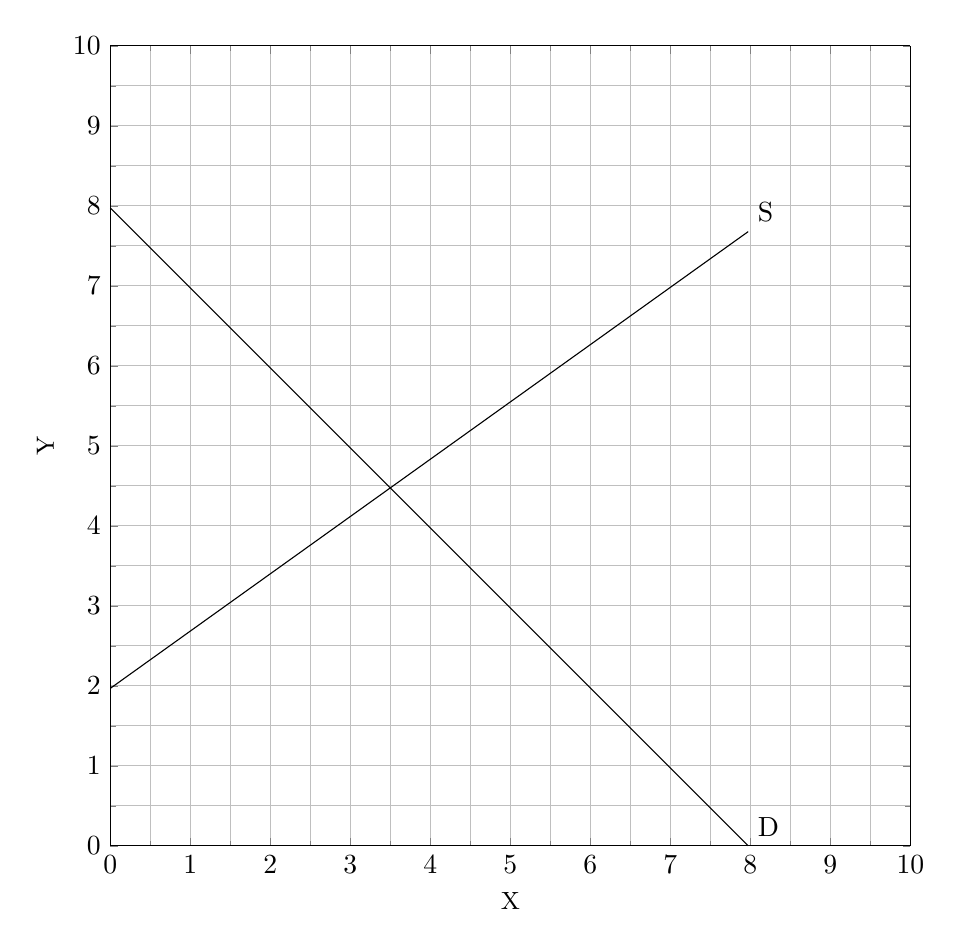
\begin{tikzpicture}
		
		\begin{axis}[%
			footnotesize,
			width=4in,
			height=4in,
			axis equal,
			scale only axis,
			separate axis lines,
			grid=both,
			every outer x axis line/.append style={black},
			every x tick label/.append style={font=\color{black}},
			xmin=0,
			xmax=10,
			xlabel={X},
			every outer y axis line/.append style={black},
			every y tick label/.append style={font=\color{black}},
			ymin=0,
			ymax=10,
			ylabel={Y},
			minor tick num=1,
			xtick distance=1,% <- 
			ytick distance=1,% <-
			axis background/.style={fill=white},
			legend style={at={(0.97,0.03)},anchor=south east,legend cell align=left,align=left,fill=white}
			]
			
		\end{axis}
		
		\draw (0,8.1) -- (8.1,0) node[above right] {D};
		\draw (0,2) -- (8.1,7.8) node[above right] {S};
	\end{tikzpicture}%
\end{center}	
}
}

%\pbn
%\exex{Exam WS-20/21}{
	%	\abcx{
		%		\item (4P) Suppose that good $A$ and good $B$ are substitutes. The market equilibrium of both goods are plotted below. 
		%	
		%	\begin{tikzpicture}[scale=.5]
			%	%	\draw [color=gray!50,opacity=0.5]  [step=10mm] (0,0) grid (10,10);
			%	%HOME	
			%	\draw[thick,<->] (0,11) node[right,font=\scriptsize]{Price}--(0,0)--(11,0) node[below,font=\scriptsize]{Quantity}; 
			%	\draw (1,10) -- (10,1) node[above right] {D};
			%	\draw (1,2) -- (9,10) node[above right] {S};
			%	\draw[] (5,12) node[left]{Good A:};
			%	%\draw[thick, red] (0,2) node[left]{$P^W$} -- (10,2)  ;
			%	\end{tikzpicture}
		%	\begin{tikzpicture}[scale=.5]
			%	%	\draw [color=gray!50,opacity=0.5]  [step=10mm] (0,0) grid (10,10);
			%	%HOME	
			%	\draw[thick,<->] (0,11) node[right,font=\scriptsize]{Price}--(0,0)--(11,0) node[below,font=\scriptsize]{Quantity}; 
			%	\draw (1,10) -- (10,1) node[above right] {D};
			%	\draw (1,2) -- (9,10) node[above right] {S};
			%	\draw[] (5,12) node[left]{Good B:};
			%	%\draw[thick, red] (0,2) node[left]{$P^W$} -- (10,2)  ;
			%	\end{tikzpicture}
		%
		%	Now, assume that intermediate goods that are needed in the production of good $A$ but not in the production of good $B$ become more expensive. Does that have an impact on supply and/or demand of good $A$ and/or $B$? If so, sketch the changes and the new equilibrium in the plots above. 
		%	
		%	\pbn
		%	\item (4P) Suppose that good $C$ and good $D$ are complements. The market equilibrium of both goods are plotted below. 
		%	
		%	\begin{tikzpicture}[scale=.5]
			%	\draw[thick,<->] (0,11) node[right,font=\scriptsize]{Price}--(0,0)--(11,0) node[below,font=\scriptsize]{Quantity}; 
			%	\draw (1,10) -- (10,1) node[above right] {D};
			%	\draw (1,2) -- (9,10) node[above right] {S};
			%	\draw[] (5,12) node[left]{Good C:};
			%	%\draw[thick, red] (0,2) node[left]{$P^W$} -- (10,2)  ;
			%	\end{tikzpicture}
		%	\begin{tikzpicture}[scale=.5]
			%	\draw[thick,<->] (0,11) node[right,font=\scriptsize]{Price}--(0,0)--(11,0) node[below,font=\scriptsize]{Quantity}; 
			%	\draw (1,10) -- (10,1) node[above right] {D};
			%	\draw (1,2) -- (9,10) node[above right] {S};
			%	\draw[] (5,12) node[left]{Good D:};
			%	\end{tikzpicture}
		%
		%	Now, assume that intermediate goods that are needed in the production of good $C$ but not in the production of good $D$ become more expensive. Does that have an impact on supply and/or demand of good $C$ and/or $D$? If so, sketch the changes and the new equilibrium in the plots above. 
		%	
		%	\pbn
		%	\item (6P) Suppose that the supplier of good $E$ decreases the price of good $E$ from \euro 119 to \euro 118. The consequence of this change is that the amount of items sold on the market decreased from 12,398 to 12,132. 
		%	\begin{enumerate}
			%		\item Can you say with certainty that this good is a\dots 
			%		\begin{itemize} 	
				%			\item \dots normal good
				%			\item \dots inferior good
				%			\item \dots giffen good 
				%		\end{itemize}
			%		\item Calculate the price elasticity of demand using the \textit{Midpoint Method}.
			%	\end{enumerate}
		%	
		%%	\item (6P) Demand and supply in a market are described by the equations
		%%	\begin{align*}
			%%	Q^D&=66-3P\\
			%%	Q^S&=-4+2P.
			%%	\end{align*}
		%%
		%%	Solve algebraically to find equilibrium price $P^*$ and quantity $Q^*$ on the market.
		%}}








%\frame{\frametitle{Solution: d)}
	%	As the price of \euro 0.60 is higher than the equilibrium price of the free market, supply will exceed demand:
	%	\begin{align*}
		%	Q^D&=30-30\cdot .6=12\\
		%	Q^S&=30\cdot .6 -3=15
		%	\end{align*}
	%	Only 12 litres of milk will be sold and total revenue is \euro 7.2:
	%	\[ \pi=12\cdot 0.6=7.2\]
	%}
%
%\frame{\frametitle{Solution: e)}
	%	\begin{align*}
		%	PED&=\frac{\frac{13.5-12}{(13.5+12)/2}}{\frac{( .55- .60)}{(.60+ .55)/2}} =\frac{\frac{1.5}{12.75}}{\frac{-0.05}{0.575}}= \frac{0.117647059}{-0.086956522}=-1.352941174
		%	\end{align*}
	%	A PED of -1.35 indicates that milk is a price-elastic good.
	%}
%






